\documentclass[en]{../../../eplsummary}

\usepackage{xurl}
\renewcommand{\indent}{\hspace{\parindent}}
\setlength\parindent{0pt}
%\setcounter{tocdepth}{3}
%\setcounter{secnumdepth}{4}

\newcommand{\inputspace}{\mathcal{X}}
\newcommand{\featurespace}{\mathcal{F}}

\usepackage{listings}
\lstset{language=Python,
    basicstyle=\small\ttfamily,
    stringstyle=\color{black},
    morekeywords={},
    deletekeywords={_},
    keywordstyle=\color{black},
    identifierstyle=\color{black},
    commentstyle=\color{DarkGreen},
    numbers=left,
    numbersep=10pt,
    showspaces=false,
    showstringspaces=false,
    showtabs=false,
    frame=single
}

\hypertitle[']{Algorithms in Data Science}{7}{INMA}{2472}
{Romain Graux\and Lionel Lamy\and Cedric Antoine}
{Jean-Charles Delvenne, Gaultier Krings, Alexey Medvedev and Rémi Delogne}


%\newpage
%\tableofcontents
%\newpage

% =============================

\section{Networks}

\subsection{Introduction}

Networks can take several forms and represent all kinds of elements (economic, biological, geographical, social, technological\dots). We will start by looking at social networks. The latter have some properties:

\begin{itemize}
    \item \textbf{Distance}: it is generally considered that social networks are small in diameter with a relatively small maximum distance between two individuals.

    \item \textbf{Triangles}: as the saying goes, ``my friend's friend is my friend''. This means that there is usually a fairly high density of triangles. In order to compute them formally we use the Clustering Coefficient:

    \[ 0 \leq CC = \frac{x \; \sharp\{\bigtriangledown\}}{\sharp\{\vee\}} = \frac{Tr(A^x)}{\sum d_i(d_i - 1)} \leq 1 \]
    The number of complete triangles on the number of triangles (empty or complete). Corresponds to the trace of the adjacency matrix $A$ on the sum of the degrees $d$ of the nodes $i$. Where $x$ is the number of sides of the triangle. In this case: 3.

    \item \textbf{Degree distribution}: the degrees are heterogeneous: there are lows and highs. We have a fat-tail. The Power Law is the fact that $\sharp\{\text{node of degree k}\} \propto k^{-\gamma}$. So if the number of nodes tends towards infinity, with $\gamma < 2$, the moments of the distribution could be infinite. If $2 \leq \gamma \leq 3$ then the mean is finite but not the variance.

    \item \textbf{Density distribution}: The density is also generally heterogeneous. There are two types: i) the community where nodes are connected in groups but almost not between groups and ii) the core-periphery where nodes are clustered on the center but less on the periphery ring.

    \item \textbf{Correlations}: Assortativity/homophily: neigbouring nodes tend to have similar meta-data (age, geographic location, etc) or structural properties (degree).

\end{itemize}

We will now discover different models and explain the different properties in a little more detail as we go along.

\subsection{Models}

\subsubsection{Erdos-Renyi}

\begin{itemize}
    \item Fix number of nodes $n$
    \item Fix number of (undirected) edges $m$
    \item We have an uniform distribution on all graphs $G(n,m)$
\end{itemize}

We might be interested by a variant (\textbf{Gilbert}) where we fix p as the probability of being friend with someone. This is interesting because we can analyze the degree distribution:

\begin{quote}
Basically, if we have a probability of becoming friends with another, then we are in the case of a binomial distribution of mean $p(n-1) \approx pn $. So, a good approximation of that is a poisson where $\lambda = pn$ and $p \ll 1$. And by the CLT the poisson itself can be approximated by a gaussian if $pn \gg 1$.
\end{quote}

We discover some new properties:
\begin{itemize}
    \item \textbf{Monotone increase property}: if you add edges, the properties are still valid.
    \item \textbf{Every monotone property has a threshold function $p^*(n)$}:

    If $\frac{p(n)}{p^*(n)} = 0$ then Prob(x) $\to 0$ and if conversely $p(n)$ is far above $p^*(n)$ we have the Prob(x) $\to 1$.

    As an exemple: for ``at least one edge'', we have the threshold function $p^*(n) = 1/n^2$.

    \[ \mathbb{E}(\#\{\text{edges}\}) = \binom{n}{2} p \sim n^2p \Rightarrow \begin{cases}
    p \ll p^* & \text{ then } \mathbb{E}(\#\{\text{edges}\}) \ll 1 \\
    p \gg p^* & \text{ then } \mathbb{E}(\#\{\text{edges}\}) \gg 1
    \end{cases}
    \]
\end{itemize}

Note that we do not have heterogeneous degrees or density or many triangles: $\mathbb{E}(\sharp\{\bigtriangledown\}) = \binom{n}{3} p^3 = \Theta\big((pn)^3\big) = \Theta\big(\bar{d^3}\big)$

The last thing to remember about ER random graph is that the diameter and average distance are close to $ln(n)$ and $ln(pn) \sim ln(d)$. Basically this act kind of an `epidemic' with $log_d n$ generations to hit the whole component.
\subsubsection{Configuration}

In order to improve the previous models and make them more realistic, several approaches are discussed.

\begin{itemize}
    \item \textbf{Fixing degree of each node}: one consider that the degree distribution is very wrong and impose a degree.
    \item \textbf{Stub model}: we randomly wire defined stubs.
    \item \textbf{Random swaps}: taking an existing network and randomly swap edges.
\end{itemize}

This configuration model is similar in many aspects to ER random graphs, for example it still have an homogeneous density and a low diameter $\log n / \log D$ where $D = \frac{\sum d_i^2}{\sum d_i}$ (but not homogeneous degree anymore).


\subsubsection{Watts-Strogatz (small world, figure~\ref{fig:watts-strogatz})}

The basic idea behind this model is that most friends live nearby but it happens that some live far-away. We start with a circle and then randomly rewire each link with a probability p. A variant is adding links instead of editing them.

This model has many triangles, a small diameter but the degrees and density aren't heterogeneous.

\begin{figure}[h]
    \centering
    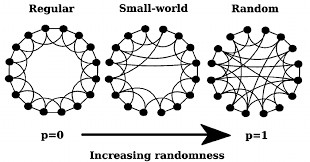
\includegraphics[width=.5\linewidth]{res/SW-Model.jpg}
    \caption{Watts-Strogatz}
    \label{fig:watts-strogatz}
\end{figure}

\subsubsection{Preferential attachment}

In this case we try to simulate the emergence of hubs (high degree nodes). ``Richs get richer'' (Matthew's effect)

This is a model of growth where at each step of time, a new node arrives and makes one connection with a probability proportional to the degree k. That means that we have a power-law degree distribution of exponent 3:
\[ \text{Prob}(\text{deg} = k) \propto \frac{1}{k^3} \]

This results in heterogeneous degree distribution and density (core, no communities) and a low diameter (even smaller) $\ln(n) / \ln(\ln(n))$, but we have only a few triangles in the end.

\subsubsection{Girvan-Newman (figure~\ref{fig:girvan-newman})}

In this model we have several densities in the same network. For example, with communities, we have a fairly high density within them and a lower density that connects them. We can extend that infinitely, ie. communities of communities.

\begin{figure}[h]
    \centering
    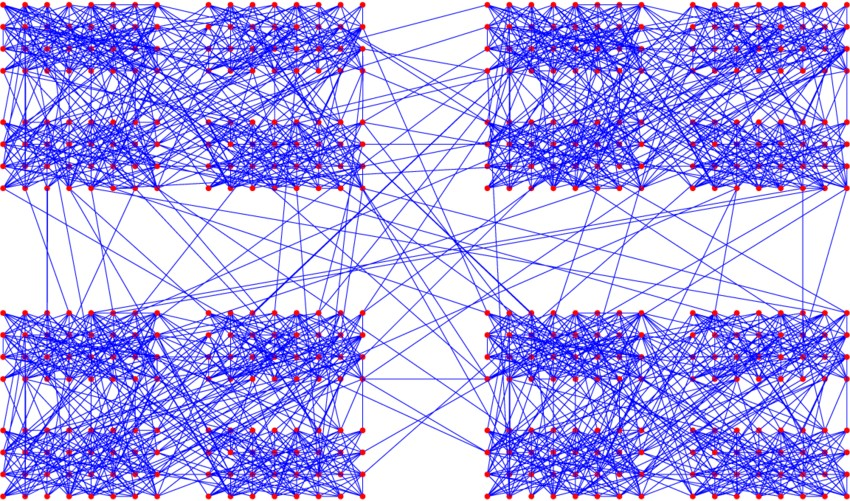
\includegraphics[width=.4\linewidth]{res/GN-Model.jpg}
    \caption{Girva-Newman}
    \label{fig:girvan-newman}
\end{figure}

\newpage
\subsubsection{Stochastic block (figure~\ref{fig:stoch-block})}
Even more general and flexible than the GN model, here we decompose the parts of the network into blocks, and for each block we say that there is a certain density.

\begin{figure}[h]
    \centering
    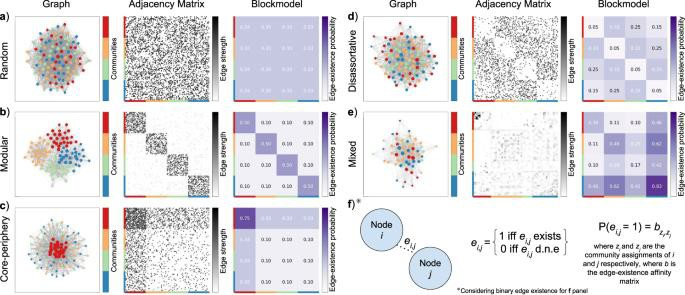
\includegraphics[width=.8\linewidth]{res/SBM-Model.jpg}
    \caption{Stochastic block}
    \label{fig:stoch-block}
\end{figure}

\subsection{Indicators of the structure}

\subsubsection{Basic}

\begin{itemize}
    \item \textbf{Degree distribution}
    \item \textbf{Clustering coefficient (recall)}:
    \[
        C_u = \frac{2T(u)}{d_u (d_u - 1)} \quad \text{ where } T(u) = \sharp\{\text{nodes linked to u} \}
    \]
    \item \textbf{Betweenness centrality}: find certain edges where each shortest path between two zones must pass through. $O(n^3)$

    \item \textbf{Closeness centrality}: find the nodes that are closest to all the others in the network. $O(n^3)$
\end{itemize}

\subsubsection{K-Core}

\textbf{Definition}: the $k$-core of a graph $G(V,E)$ is its maximal subgraph $G'(V',E')$ such that all nodes of $G'$ have a degree $\geq k$.

Scales linearly with the number of links in the network. Only applicable on undirected networks, and works best on unweighted networks. There exists a version for weighted networks, but it requires arbitrary thresholds. All nodes in the $k+1$-core are contained in the $k$-core. The largest possible core is therefore given by the maximal degree in the graph. The difference between the $K+1$-core and the $K$-core is called the $K+1$-shell.

The idea behind the algorithm is the following [Complexity time $\bigoh(m)$ and space $\bigoh(n+m)$]:

\begin{lstlisting}
while every node has not been pruned:
    to_prune = list(nodes of degree k)
    k_shell = empty_list()

    while to_prune is not empty:
        x = first elem of to_prune
        for each neighbor of x:
            if it is not pruned:
                decrease by 1 its degree
                if its degree is now k: add to the list to_prune
        x is now pruned
        add x to k_shell
        increase total_pruned by 1

    store k_shell and do the same for k + 1
done
\end{lstlisting}

\subsubsection{S-Core}

S-core decomposition works exactly the same as $k$-core, except that we replace the degree of each node by its weighted degree $s$ (the sum of the weights of its edges). If the link weights are diverse, the risk is, however, that we end up with each node in one core. A possible outcome for that is to create thresholds for defining cores, but unless there those can be linked to a concrete meaning, it's difficult to have an objective way to separate those. Intervals are commonly used.

\subsection{Nodes with metadata}

\subsubsection{Assortativity}
``Birds of a feather flock together''

\begin{itemize}

\item \textbf{Scalar node labels}

Assume that we are in a simple graph and that every node has a scalar label (eg. age, degree, salary\dots). We can pick a random edge and call the extremities X and Y: the assortativity coefficient of the label is $\text{Corr}(X,Y)$. (Newman)

\item \textbf{Binary labels}

If instead of labels we have binary categories (gender, smoker\dots) and want to know how many of our friend belongs to a certain one, we replace the label by $-1$ and $1$ and compute, with m the nb of edges and $\mathcal{L}$ the label:
\[
BA_\mathcal{L} =
\frac{
    \frac{
        |\text{Edges between same label}|
        }
        {m}
        - \sum_{\mathcal{L}} p^2_\mathcal{L}
    }
    {
    1-\sum_{\mathcal{L}} p^2_\mathcal{L}
    }
\]

\item \textbf{Categorical labels}: same as BA formula.

\item \textbf{Non-simple graphs}: we consider weight as multiplicity of edge, and the probability of edge being chose is proprotional to weight. For directed graph, we must dinstinguish origin (X) and target (Y). (replacing $p^2_\mathcal{L}$ by $p_\mathcal{L}q_\mathcal{L}$)

\end{itemize}
Be careful that the weighting is done on the number of degrees. Therefore, in the calculation the nodes of high degree will count more. This is not really a `democratic' measure. Moreover, an assortativity of $+1$ is only possible for disconnected graphs and $-1$ for bipartite one. Plus, assortativity behaviour can be non uniform across large network.

\subsection{Community detection}

Community detection methods group nodes in highly-connected clusters, based on some objective functions. This allows to unfold the global organisation of nodes in clusters and make higher-order and finer analyses. However, it is not always possible or necessary to find a community.

One of the first idea (by Kerger-Stein) was to find the absolute min cut (how many relationships to form a community if I got it right) but was too computer intensive for often trivial result. Shi-Malik then added a regularisation for promoting same-size communities. Given k, the number of communities as an input, and with k = 2:
\[ \text{Ncut} = \text{Cut}\Big(\frac{1}{\sum_{i \in C_1}d_i}+\frac{1}{\sum_{i \in C_2}d_i}\Big) \]

\subsubsection{Modularity}
In this case we are trying to find out if the connections between nodes are higher than what could be expected on average in a random network. The number of edges expected in, for example, a config model inside a set of nodes C is:

\[ \sum_{i,j \in C}\frac{d_id_j}{2m} \approx \mathbb{E}\big(\sharp \text{ edges between i and j}\big) \]

Basically that's the probability that they connect together. So the modularity is the number of edges inside a supposed community minus the expected number of edges, the whole normalized (to be into $[-1 ; 1]$). If we have a positive modularity, that means that we have more internal connections than expected.

\[ M = \frac{1}{2m} \quad \sum_{i,j \in \text{Same community}} \quad A_{ij} - \frac{d_id_j}{2m} \]

It can also be seen as a min-cut problem regularised with term promoting diversity (many equal-sized communities).

\[ 1 - \frac{\text{Cut}}{m} - \sum_{C} p^2(C) \quad \text{with} \quad p(C) = \sum_{i\in C} \frac{d_i}{2m} \]


\subsubsection{Algorithms}
%\todo[inline, backgroundcolor=orange!45]{$\;$ To redo, it is neither comprehensive nor complete. I suggest you to look at the slides while watching the replay.}

\begin{itemize}
    \item \textbf{General heuristics}: try to tackle the NP-hardness to maximise goodness criterion like NCut or Modularity. We use local search (swaps by Kernighan-Lin) or simulated annealing (but slow). \textit{No more info}.

    \item \textbf{Spectral methods}: another popular method quite efficient. That's essentially a matrix representation of networks. There exists several ways to do that like Adjacency matrix, Modularity matrix and (Normalized) Laplacian. The latter is constructed as follow: $L = D - A$ with $D$ the diagonal matrix of degrees and A the adjacency matrix (figure~\ref{fig:spectr-laplacian}).
    \begin{figure}[h]
        \centering
        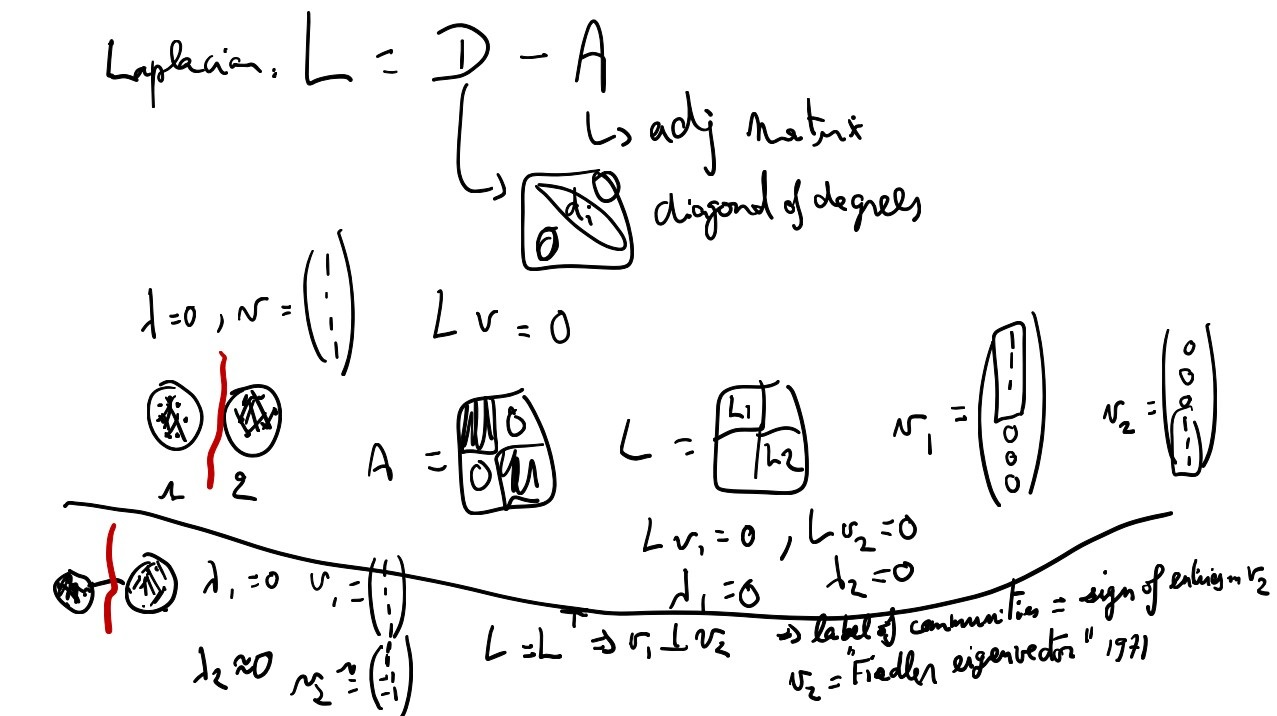
\includegraphics[width=.7\linewidth, height=6cm]{res/Laplacian.jpg}
        \caption{Idea of the spectral method with the Laplacian}
        \label{fig:spectr-laplacian}
    \end{figure}

     The Normalised Laplacian is $NL = D^{-1/2} L D^{-1/2}$

    \item \textbf{Combinatorial methods}

    \item \textbf{Louvain method}: (Blondel, Guillaume, Lambiotte, Lefèvre, 2008, figure~\ref{fig:louvain-method})

    The inspiration for this method of community detection is the optimization of modularity as the algorithm progresses. One start from individual nodes as communities and for each node in turn, try merging it with other communities if it improves the modularity. Then each small community is grouped into one node and the first step is repeated. This method is \textbf{fast and random} (order in which nodes are considered changes) so we can test the robustness of the partition found by re-running and look distance/dissimilarity. For instance one use \textbf{Jaccard index}.

    \begin{figure}[h]
        \centering
        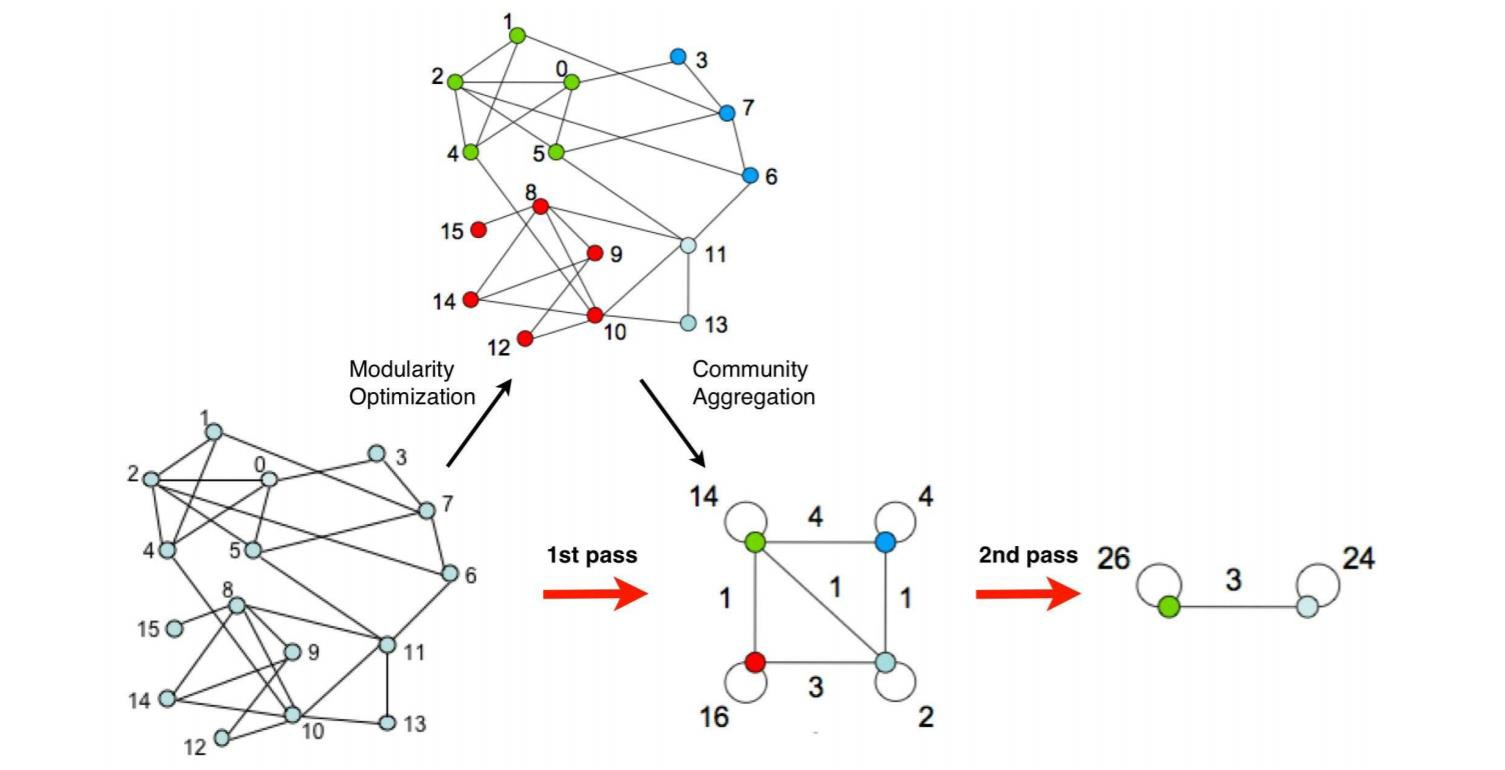
\includegraphics[width=.6\linewidth, height=5.5cm]{res/Louvain-algo.jpg}
        \caption{Louvain method}
        \label{fig:louvain-method}
    \end{figure}
\end{itemize}

\subsection{Diffusion processes}

\subsubsection{Mathematical epidemiology}
Compartmental models: population is divided in compartments based on their health status. (Bernoulli in 1760 then 20th)

They describe a variety of diseases, assume populations are homogeneously mixed and rely on parameters:
\begin{itemize}
    \itemsep0em
    \item $\beta$: average number of adequate contacts (i.e. contacts that make a transmission) for 1 individual for 1 time-step
    \item $1/\gamma$: average duration of the infectious period
    \item $1/\epsilon$: average duration of the latent period
    \item $1/\delta$: average duration of the passive immunity
\end{itemize}

\subsubsection{Linear threshold model (LTM)}

Used in modelling of diffusion of innovation/ideas and ``the spread of influence''. Type SI (stay infected).

Given a graph $G(V,E)$: Each edge $(u, v)$ is assigned a weight $w_uv$, such that for every node $u$, $\sum_v(w_{vu}) \leq 1$.

Then, each node $u$ chooses a threshold $\theta_u$ uniformly between 0 and 1. $\theta_u$ represents the weighted fraction of neighbours of $u$ that are required to activate $u$. At every step, if $\sum_{\text{v in activated nodes}}(w_{vu}) \geq \theta_u$, then $u$ becomes active.

\subsubsection{Independent cascade model (ICM)}

Animation here: \url{https://github.com/RomainGrx/LINMA2472-Homeworks/blob/main/miscellaneous/animations/cascade.gif}.
With a set $A0$ of activated nodes at the start, at every step if a node $u$ becomes activated it makes a single attempt to try to infect its neighbours $v$ which succeeds with probability $p$ (independent of past trials).
The process stops when no more nodes can be infected.
We can perform link percolation: random removal of links in a graph, and study the size of the connected components that are left.

\subsubsection{On transport networks}
\subsubsection{Influence of structure on diffusion of ideas}

The degree heterogeneity influences the spread of information on networks. The number of expected activated nodes at the first step is the same for both graphs: it is the average degree times the conversion probability. However, the degree of the nodes that are activated at the next steps have a higher expected degree than the average degree of the graph, particularly in heterogeneous networks.

\subsubsection{Limiting the spread of an epidemic}

Limiting the spread of an epidemic can be worked on two levels:
\begin{enumerate}
	\item Reducing the risk of contagion: adoption of guidelines
	\item Limiting the possible transmission paths by vaccination or limitation of social contacts.
\end{enumerate}
This is impacting the structure of the social network, and is related to percolation theory.

Some strategies of node percolation can very efficiently decompose a graph. If we cut the links in the network, that would reduce its connectivity. Practically we see this in reality with social bubble and confinement.

\subsubsection{Maximizing the spread of information}

Given a graph $G(V,E)$, we define the influence of a set of nodes $A$ as $\sigma(A)$ = the expected number of active nodes at the end of the diffusion process given that $A$ is the initial set of active nodes. Then, we define the Influence Maximization Problem (IMP) as, for a given $k$, finding the set of size $k$ with maximal influence. Problem: for the ICM and the LTM, the IMP is NP-hard. The influence function of a set of nodes $\sigma(A)$ is submodular (shows property of diminishing returns), non-negative and monotone.

\subsubsection{Greedy hill-climbing heuristic}

\begin{lstlisting}
AO = empty_list()
X = generate a large number of graphs with some randomly activated edges

until we have k best nodes:
    for each node not in AO:
        for each graph in X:
            score by its number of accessible neighbors
        sum up its global score (across all realisations X)
    add the node with the best score to AO
done
\end{lstlisting}

The heuristic performs better than targeting high degree nodes, but comes with a computational cost. More pragmatic approaches exist to avoid computational issues like social leader detection: a node $u$ is a social leader if it has a higher social degree than all its neighbours.

% =============================
\section{Embeddings}

\begin{itemize}
    \item An embedding is a representation of the set of instances in a (relatively) low dimensional space, that preserves some information about the instances from the original space.
    \item An embedding algorithm takes high-dimensional data and maps it to the lower dimensional space.
    \item The algorithm must be designed to keep as many features of the high dimensional data in the lower dimensional world after the mapping operation.
\end{itemize}

\subsection{Principal components analysis (PCA)}

PCA is a dimension reduction method that tries to reduce dimensionality by maximising the variance of the the data projected on the low dimensional space. Thus, it will keep the directions of the most important variables.

\subsubsection{How it works}

%\begin{itemize}
%    \item Center data $X_c=(I_n - \dfrac{1}{n}11^T)X$
%    \item Compute the covariance matrix $Z = X_c^T X_c$
%    \item Compute the eigen decomposition of $Z = U\Sigma U^{-1}$
%    \item Keep the N higher eigenvalues and eigenvectors $V$
%    \item Project the data on the new space $X^* = X V$
%\end{itemize}

\begin{itemize}
    \item Center data $X_c=(I_n - \dfrac{1}{n}11^T)X$
    \item Compute the singular value decomposition $X_c = \mathcal{U}\Sigma\mathcal{V}^T$
    \item Keep the $N$ biggest singular values and singular vector column corresponding $\mathcal{V}_h$
    \item Then you can obtain the project data with $y = \mathcal{V}_h^T X$
\end{itemize}


\subsubsection{Pros}

\begin{itemize}
    \item Easy to compute
    \item Removes Correlated Features
\end{itemize}

\subsubsection{Cons}

\begin{itemize}
    \item Can only compute linear correlation dependance
\end{itemize}


\subsection{Auto-encoders}

An autoencoder is a type of artificial neural network (ANN) used to learn efficient data codings in an unsupervised manner. The aim of an autoencoder is to learn a representation (encoding) for a set of data, typically for dimensionality reduction, by training the network to ignore signal ``noise''. Along with the reduction side, a reconstructing side is learnt, where the autoencoder tries to generate from the reduced encoding a representation as close as possible to its original input, hence its name.

\begin{figure}[H]
    \centering
    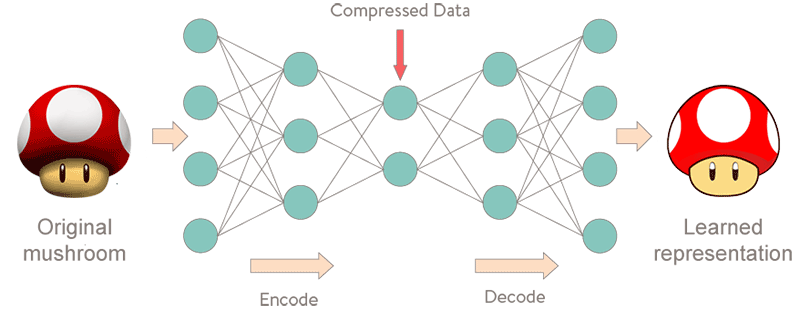
\includegraphics[width=.8\textwidth]{res/autoencoder.png}
    \caption{Auto-encoder structure}
    \label{fig:autoencoder}
\end{figure}

\subsubsection{Artificial neural networks}

To understand how an auto-encoder works, we need first to understand how an ANN is trained. An ANN needs several parts to be able to learn: \textit{neurons}, \textit{loss function}, \textit{backpropagation}.

\vspace{1em}

\textbf{Neurons}

A neuron is a single entity that receives many signals as input and output a scalar, it is composed of weights and an activation function. To reduce the input signals as a scalar, each input signal is added with a corresponding weight and we finally add a \textit{bias}. Before being output, the output signal go to an activation function (ReLU, Sigmoid, Linear\dots) to finally obtain $y = \varphi(w_1 x_1 + \dots  + w_n x_n + b)$.

\begin{figure}[H]
\centering
\begin{minipage}{.5\textwidth}
  \centering
  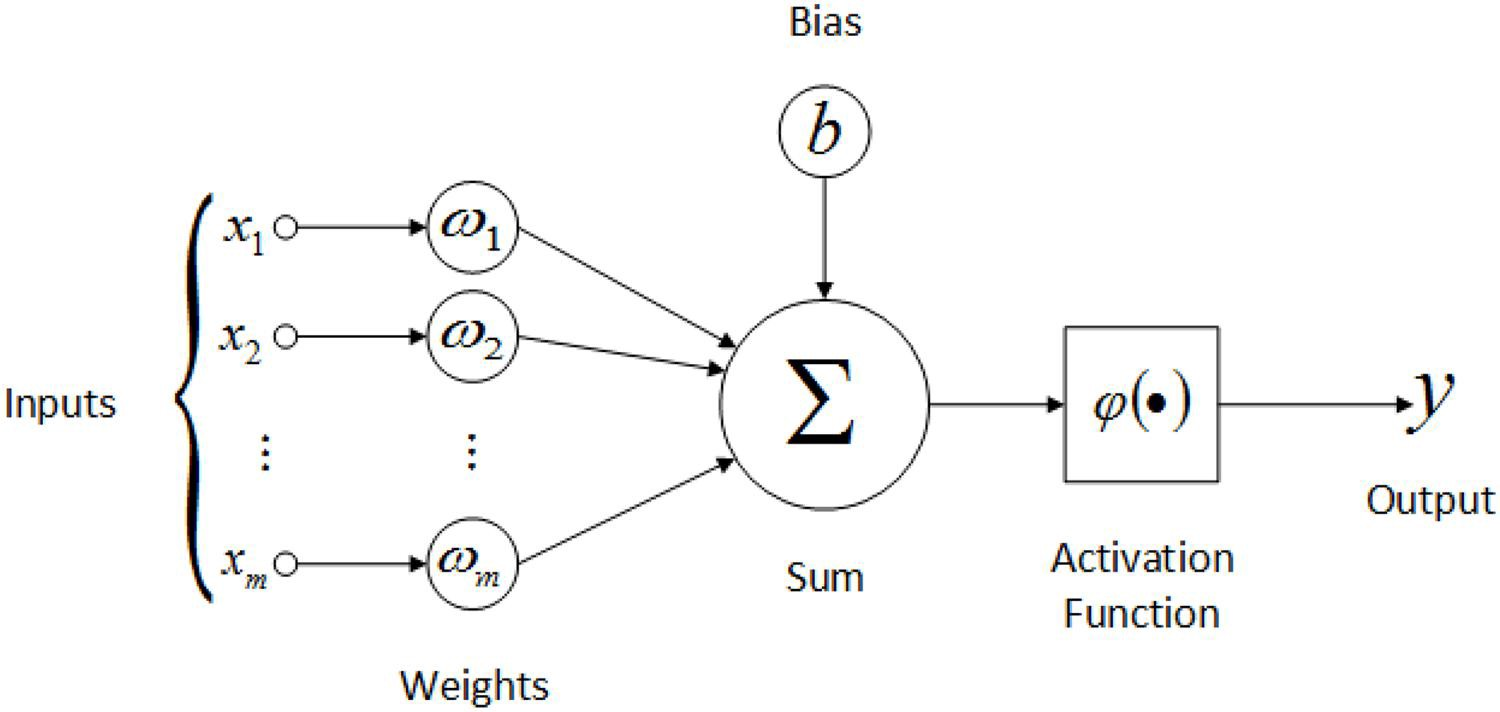
\includegraphics[width=.85\linewidth]{res/neuron.jpeg}
  \captionof{figure}{Neuron structure}
  \label{fig:neuron}
\end{minipage}%
\begin{minipage}{.5\textwidth}
  \centering
  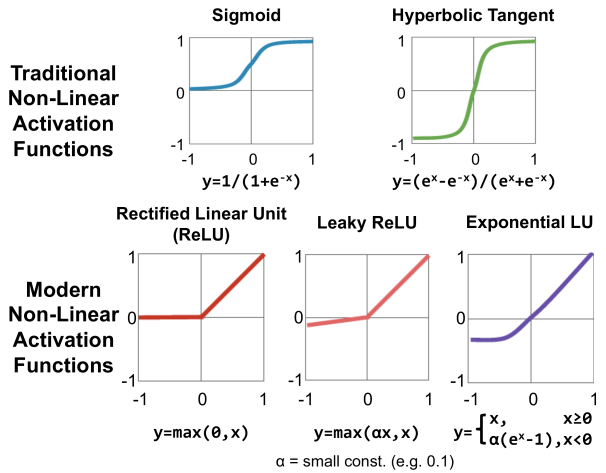
\includegraphics[width=.85\linewidth]{res/activation.png}
  \captionof{figure}{Several activation functions}
  \label{fig:activation}
\end{minipage}
\end{figure}

\vspace{1em}

\textbf{Loss functions}

A loss function is used to quantify the error of network and then adjust the weights as we will see in~\ref{pt:backprop}.

\vspace{1em}

\textbf{Backpropagation}\label{pt:backprop}

To learn, an ANN use a gradient descent approach and thus need to compute those gradients to be able to change the weights. To do this, from the loss function (scalar), each weight gradient is computed in a backward pass (cascade layer per layer in the backward direction). Finally we can change the weights with the computed gradients and that is what is called \textit{backpropagation}.

\vspace{1em}

\textbf{Training dangers}

Several difficulties can be faced with the ANN, here is an non-exhaustive list:

\begin{itemize}
    \item \textbf{Undefitting}: too little training meaning bad generalisation of the model.
    \item \textbf{Overfitting}: too much training can also lead to bad generalisation. In that case the network will perform well on the training data but not on new unseen data.
    \item \textbf{Plateau}: Slow learning (plateau), potentially leading to underfitting: In neural networks a bad choice of activation functions can lead to plateaus on the error surface. Gradient methods then become extremely slow due to the flatness of the error curve (for more info, see Vanishing gradients).
\end{itemize}

\vspace{1em}

How to avoid overfitting:
\begin{itemize}
    \item \textbf{Early stopping}: Stop training when the test error starts to rise.
    \item \textbf{Regularisation ($L_1$, $L_2$ \text{and} Elastic Net}: Statistical method that penalises the weights.
    \item \textbf{Dropout}: Force a random number of neurons to ``turn off'' during each training stage, forcing the signal to spread through the whole network.
\end{itemize}

There are a lot of parameters such as: Number of layers, Number of neurons, Optimizer (SGD, Adam, RMSProp\dots), Initial weights, Activation functions, Learning rate\dots
And a bad parameter in any of the above could screw up the whole network!

\subsubsection{Auto-encoder}

The auto-encoder is thus a neural network composed of those blocks but with a particular shape: as you can see on the Figure~\ref{fig:autoencoder}, the encoder has a bigger input space then the output space and the decoder is the opposite.

\vspace{1em}

Mathematically, we can reprensent the auto-encoder as:

\begin{itemize}
    \item $x_i \in \inputspace$, where $\inputspace$ is the \textit{Input Space}.
    \item $h \in \featurespace$, where $\featurespace$ is the \textit{Feature Space} and $h$ is the latent variable that represents $x_i$ mapped in $\featurespace$.
    \item $\phi\colon \inputspace \mapsto \featurespace$ the function that maps an instance $x_i \in \inputspace$ to $h \in \featurespace$ (Encoder)
    \item $\psi \colon \featurespace \mapsto \inputspace$ the function that maps $h \in \featurespace$ to $x' \in \inputspace$ (Decoder)
\end{itemize}

And the whole process can be discribed as
\begin{align*}
h &= \phi(x) \\
x' &= (\psi \circ \phi)(x) \\
\hat{\phi}, \hat{\psi} &= \argmin_{\phi,\psi} \norm{x - (\phi \circ \psi)(x)}^2
\end{align*}

If we use a Mean Squared Error as loss function.

\subsubsection{Link with PCA}

Recall the PCA obtains the low dimensionnal vector $y$ as $\mathcal{V}_h^T X$ and we can recover the reconstructed input as $\hat{X}= \mathcal{V}_h \mathcal{V}_h^T X$.

\vspace{1em}

So the PCA is just a particular case of an auto-encoder with $\phi = \mathcal{V}_h$ and $\psi = \mathcal{V}_h^T$.

\vspace{1em}

So, the difference is that PCA computes linear projection on the space that maximises the variance of the data on each new axis when an auto-encoder computes non-linear projection (thanks to the activation functions) and tries to be able to reconstruct the input from the \textit{Feature Space}.

\subsection{Word embedding}

Word embedding is the process of mapping each word in a $\mathbb{R}^n$ space (embedding/feature space) such that similar words are close in the \textit{Feature Space} and opposite words will be far away.

\subsection{Word2Vec}

Given a text corpus the model trains a neural network to produce the word embedding based on its context in the document.

\begin{figure}[H]
    \centering
    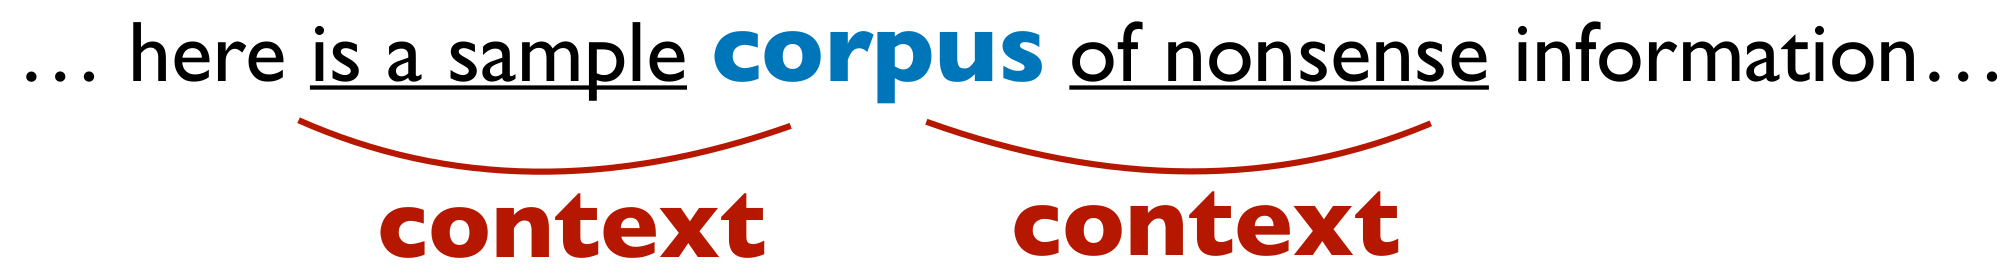
\includegraphics[width=.5\textwidth]{res/context_corpus.png}
    \label{fig:context_corpus}
\end{figure}

\subsubsection{Continuous Bag of Words (CBOW)}

\begin{minipage}{.6\textwidth}

\textbf{Input}: context of around the word

\textbf{Output}: predict the target word

The purpose is to predict the target word from its context.

\end{minipage}
\begin{minipage}{.3\textwidth}
\begin{center}
    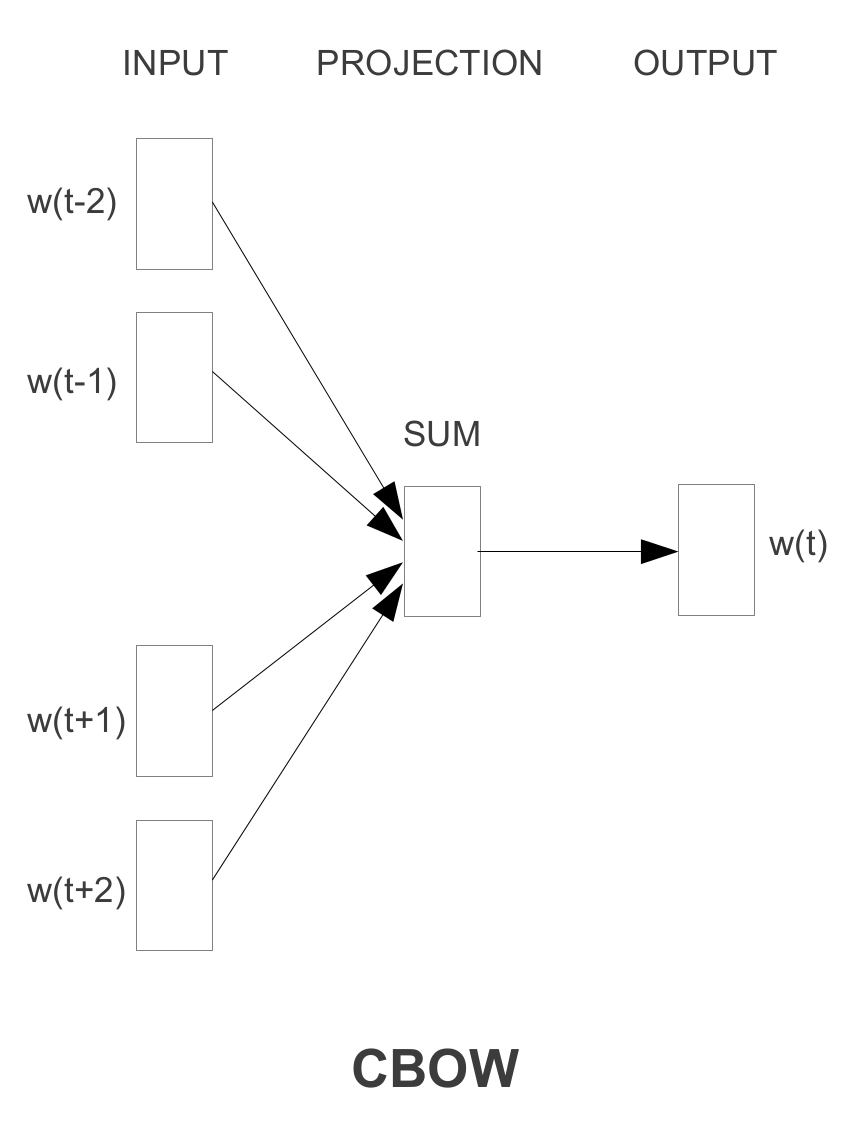
\includegraphics[width=\linewidth]{res/cbow.png}
\end{center}

\end{minipage}

\subsubsection{Skip-gram}

\begin{minipage}{.6\textwidth}

\textbf{Input}: target word

\textbf{Output}: predict the context of the target word

The purpose is to predict the context receiving the target word as input.

\end{minipage}
\begin{minipage}{.3\textwidth}
\begin{center}
	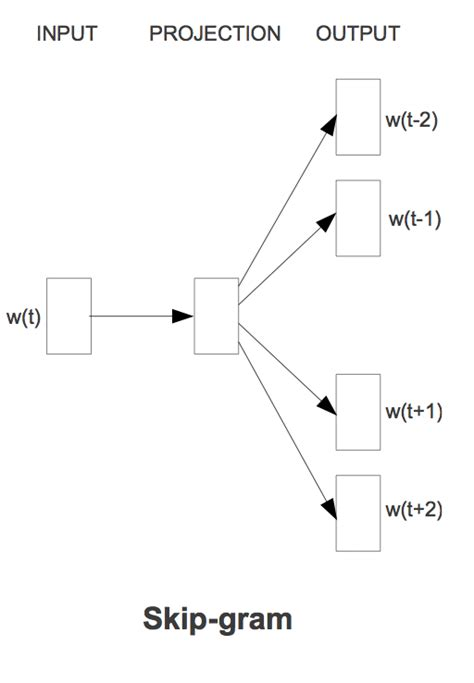
\includegraphics[width=\textwidth]{res/skip.jpeg}
\end{center}
\end{minipage}

\subsection{Node2Vec}

Node2Vec is an algorithmic framework for representational learning on graphs. Given any graph, it can learn continuous feature representations for the nodes, which can then be used for various downstream machine learning tasks (Community detection, layouts\dots).

\subsubsection{Random walks}

Random walk on a network $G = (V, E)$:

\begin{itemize}
    \item fix the probabilities P($i \rightarrow j$) to jump from any node $i$ to any neighbouring node $j \in N(i)$;
    \item place a walker on the node $u \in V(G)$ ;
    \item perform the jump according to $P(u \rightarrow v_j)$
    \item update $u \coloneqq v_k$ and go to step 3
\end{itemize}


Given a graph $G=(V, E, W)$, the random walk jump probabilities are given as follows (figure~\ref{fig:rw}).

\begin{itemize}
    \item start at a node $t \in V$;
    \item probability of the first jump is proportional to the weight of an edge $(t, v)$;
    \item next jumps: probability is proportional to the weight $W$ and the coefficient $\alpha$, which equals:
    \begin{itemize}
        \item $\frac{1}{p}$: if an edge leads to the previous node;
        \item $\frac{1}{q}$: if an edge leads to an unexplored node;
        \item $1$: else.
    \end{itemize}
\end{itemize}

\begin{figure}[H]
    \centering
    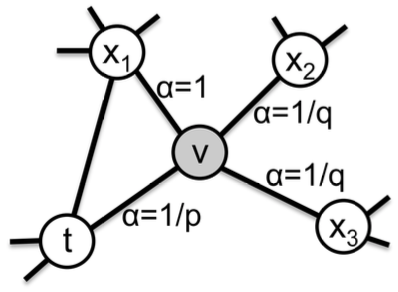
\includegraphics[width=.25\textwidth]{res/rw.png}
    \caption{Random walk}
    \label{fig:rw}
\end{figure}

\subsubsection{How it works}

Algorithm:

\begin{itemize}
    \item $\forall v \in V$ generate $N$ walks from $v$ of length $d$ (cropus);
    \item train Word2Vec model on this corpus.
\end{itemize}

Output: node embedding into the vector space based on the proximity in the random walk.

\subsection{GLoVe (2014)}

Based on the co-occurence matrix of words in a corpus.

The training objective is

\[ \exp(u v^T) \sim \text{P(word }u | \text{word } v\text{)} \]

\vspace{1em}

\textbf{Advantage}: slightly better than Word2Vec.

\vspace{1em}

\textbf{Problems}: No fine tuning, no transfer learning and no context.


\subsection{ELMo (2017)}

GLoVe was not using the context but the embedding needs to be contextual (a same word can have several meanings).

\vspace{1em}

ELMo is using Long Short Term Memory (LSTM) that is a type of recurrent neural network that is able to remember a certain amount of previous input. The task is to predict the next word with the previous context.

\vspace{1em}

\textbf{Advantage}: pre-training, contextual.

\vspace{1em}

\textbf{Problems}: No transfer learning and LSTM is sequential (no parallelisation).

\subsection{Transformer (2017)}

Transformers are using \textbf{Attention mechanism} to learn three vectors from each input: \textit{Query}, \textit{Key}, \textit{Value}.

\subsubsection{Attention }

Attention is used to focus more or less to certain part of the input instead of setting all part of the input as important.



\subsection{Bidirectional Encoder Representations from Transformers (BERT (2018))}

2 ideas:
\begin{itemize}
    \item Pre-train the general purpose language model
    \begin{itemize}
        \item Prediction of masked words
        \item Next sentence prediction (tell if a sentence B is the next sentence regarding to sentence A)
    \end{itemize}
    \item Fine tune it later for a specific task
\end{itemize}

\vspace{1em}

\textbf{Advantage}: State-of-the-art, transfer learning, embedding of sentences.

\vspace{1em}

\textbf{Problems}: word embedding is ambiguous.

%\subsection{Text processing}
%
%\todo[inline, backgroundcolor=orange!50]{TODO : finish before the exam :)}



% =============================
\section{Privacy}

\subsection{What is privacy and why (we think) it matters in today's world}

\subsubsection{Modern privacy}
Don't fall in the common fallacy that privacy is about data not being collected or
shared. Modern (informational) privacy is about the individual having (meaningful)
control over information about them, including when it's used against them. Even after the information has been disclosed, the right to erasure or right to be forgotten remains. A lot of laws worlwide are protecting privacy.

\subsubsection{Why privacy (still) matters}
\begin{enumerate}
    \item It is a basic human right:
    \begin{itemize}
        \item No one shall be subjected to arbitrary interference with his privacy, family, home or correspondence, nor to attacks upon his honor and reputation.
        \item Everyone has the right to the protection of personal data concerning him or her.
    \end{itemize}
    \item There is no freedom of thought without privacy:
    \begin{itemize}
        \item The right to privacy is often understood as an essential requirement for the realization of the right to freedom of expression.
    \end{itemize}
    \item The ``nothing to hide'' argument is flawed on many levels:
    \begin{itemize}
        \item Sometimes you want to be let alone even if you're doing nothing bad. That's why we have doors.
        \item Privacy is essential to protect freedom and dignity against fear of shame.
        \item The ``nothing to hide'' argument implicitly assumes that there are only two kinds of people: good citizens and bad citizens. But are dissidents bad? And whistle-blowers? And journalists? Bad according to who and when?
    \end{itemize}
    \item Chilling effect and access to information:
    \begin{itemize}
        \item When people know they are being (or might be) watched, they behave differently. This is this idea behind Jeremy Bentham's Panopticon (\textit{design that allow all prisoners of an institution to be observed by a single security guard, without the inmates being able to tell whether they are being watched.}).
    \end{itemize}
\end{enumerate}

\subsection{Terminology}
\begin{itemize}
    \item \textbf{Sensitive information} = a piece of information about an individual (e.g. disease, drug use) we're trying to protect (but is relevant for the application).
    \item \textbf{Identifier} = A piece of information that directly identifies a person (name, address, phone number, ip address, passport number, etc)
    \item \textbf{Quasi-identifier} = A piece of information that does not directly identify a person (e.g. nationality, date of birth). But multiple quasi-identifiers taken together could uniquely identify a person. A set of quasi-identifiers could be known to an attacker for a certain individual (auxiliary info).
    \item \textbf{Auxiliary information} = Information known to an attacker.
    \item \textbf{Uniqueness} = fraction of the dataset that is uniquely identified by the set A of quasi-identifiers
\end{itemize}


\subsection{Data pseudonymization and anonymization}
\begin{itemize}
    \item \textbf{Anonymization} = disassociating an individual's record from their identity in a particular dataset.
\end{itemize}

In short: if the data is anonymous it is not personal data anymore $\Rightarrow$ no consent, no purpose.

\begin{itemize}
    \item \textbf{Pseudonymization} = removal of direct identifiers (name, phone number, address, social security number\dots) and just give each person a unique id that cannot be linked to them.
\end{itemize}

Pay attention that pseudonymized data is not necessarly anonymous!

\subsubsection{How to pseudonymize data}
\begin{itemize}
    \item We could build a correspondence table between direct identifiers and random generated strings but:
    \begin{itemize}
        \item It quickly becomes cumbersome to save it and keep it up-to-date as new data arrives
        \item We need to make sure the strings are unique (collisions)
    \end{itemize}
    \item We could use a secret formula (e.g. for phone number: pseudonymized ID = phone number * 17 + 12345) but:
    \begin{itemize}
        \item If somebody knows the real phone numbers of a couple of people in the dataset it's easy to find back the formula (even with complex functions)
        \item And \textbf{collisions} are also an issue
    \end{itemize}
    \item A good idea is to use `cryptographic hash functions' but:
    \begin{itemize}
        \item If an attacker were to know which hash function we used and the size of our input space, they can easily build a lookup table by iterating over all possible IDs! (a brute-force attack)
    \end{itemize}
\end{itemize}
Solution to make inversions actually impossible: salt hashes!
\begin{itemize}
    \item \textbf{A salt} = fixed string of arbitrary length (but long!) that is added to the identifier before hashing it. Note: the salt must be kept secret.
\end{itemize}

\subsubsection{How to anonymize data}

In general, re-identification attacks leverage the uniqueness of individuals in the dataset. We can use k-anonymity to fight uniqueness (uniqueness attack).

\begin{itemize}
    \item A table is \textbf{$k$-anonymous} if every record in the table is indistinguishable from at least $k-1$ other records, with respect to every set of quasi-identifiers
\end{itemize}

This means that even if an attacker knows all possible quasi-identifiers, she cannot identify his target uniquely.

\vspace{1em}

How to achieve k-anonymity:
\begin{itemize}
    \item Non-perturbative methods (data truthfulness):
    \begin{itemize}
        \item \textbf{Generalization}: replacing attribute values with more general ones
        \item \textbf{Suppression}: deletion of a column (attribute) or a row (individual)
    \end{itemize}
\end{itemize}

\begin{itemize}
    \item Perturbative methods:
    \begin{itemize}
        \item \textbf{Noise addition}: gaussian noise
        \item \textbf{Data swapping}: swap attributes between individuals
    \end{itemize}
\end{itemize}

Other methods to anonymize are:
\begin{itemize}
        \item \textbf{Achieving $l$-diversity}. An equivalence class is $l$-diverse if it contains at least $l$ distinct values for the sensitive attributes. A table is $l$-diverse if every equivalence class is $l$-diverse.
        \item \textbf{Achieving $t$-closeness}. An equivalence class is said to have t-closeness if the distance between the distribution of a sensitive attribute in this class and the distribution of this attribute in the whole table is no more than a threshold $t$. A table is said to have t-closeness if all equivalence classes have $t$-closeness.
    \end{itemize}

But even this methods can sometimes not be enough.

\subsubsection{Some attacks examples}
\begin{itemize}
    \item \textbf{A homogeneity attack} can take place when individuals in the same equivalence class all have the same sensitive attribute value (use l-diversity to prevent this)
    \item \textbf{A semantic attack} can take place when sensitive attributes of individuals in an equivalence class are distinct but semantically similar. (e.g. different cancers) (use t-closness to prevent that)
    \item \textbf{A skewness ``attack''} (here it is probabilistic) takes place when the distribution of the sensitive attributes in a class is skewed. In the general population, 99\% might test negative for illegal drugs but, in an equivalence class, only 15\% test negative. I learned something about people in this class. (use t-closness to prevent that)
\end{itemize}

\subsubsection{Preserving utility of data}

Anonymizing the dataset intrinsically requires you to make the information less precise, complete, and/or accurate. This is an issue when researchers are then trying to use the data.

\vspace{1em}

People use \textbf{entropy} to measure the amount of information left in the dataset and the loss of information resulting from anonymizing the dataset.

\[ \text{Entropy} = -\sum_{i=1}^{k} \frac{\#C_i}{N} \log\frac{\#C_i}{N} \]

Where: N is the amount of rows in the dataset D;
$C_1, \dots, C_k$ are the equivalence classes; $\#C_i$ indicates the number of rows that belong to $C_i$. The higher the entropy, the more information is contained in D.

\vspace{1em}

We can add that utility also depends on the use of the data.

\subsection{Big Data anonymization}

\subsubsection{What is Big Data}

Formally (according to Google): ``extremely large data sets that may be analysed computationally to reveal patterns, trends, and associations, especially relating to human behaviour and interactions.''

\vspace{1em}

In short the data is:
\begin{itemize}
    \item Large and often high-dimensional (``lots of columns''), it does not fit in Excel.
    \item Automatically collected as a side-effect of our technology.
\end{itemize}

For Big data the standard terminology, assumptions, and metrics do not work anymore.

\vspace{1em}

The data corresponds to a behavioural trace of an individual:
\begin{itemize}
    \item There is no sensitive attribute: every point in the data is potentially sensitive.
    \item There is no quasi-identifier: no point or combination of points that clearly identifies every individual (and can be assumed to be known by an adversary).
\end{itemize}

Hence, the standard definitions of small scale data anonymization does not work anymore. We need new definitions and metrics.

\subsubsection{From uniqueness to unicity ($\epsilon_p$)}

No quasi-identifiers or sensitive data anymore, every point is both sensitive and a point that could be known to an attacker. However, we don't assume an attacker knows all the points, just a few (p) of them. Unicity aims at quantify the risk of re-identification in large scale behavioural datasets.

\vspace{1em}

Formally:
\begin{itemize}
    \item \textbf{unicity} ($\epsilon_p$) of a dataset = the average fraction of the users in the dataset that are uniquely identified by p random points in their trajectory
\end{itemize}

Estimating unicity exactly would take a very very long time, one would need to compute for all users (n = 1.5M ) and for all set of points from their traces (~1000 depending on the chosen p) whether this makes them unique or not. (mobile phone metadata example)

Instead, we used the following procedure that relies on:
\begin{itemize}
    \item A random set of 10000 users
    \item For which we draw p points at random
    \item And whether these points make them unique
\end{itemize}

An attacker can could collect points about us offline but also online (we constantly broadcast our location on many services like facebook or twitter).

\vspace{1em}

\textbf{What does unicity tell us about behavior:}

\vspace{1em}

Unicity measures what distinguishes one
person from literally everybody else in the
dataset.E.g.:

\vspace{1em}

Looking at unicity in credit card data we
showed that:
\begin{itemize}
    \item Women are easier to identify than men. (Odds of women to be unique is 1.214 times greater than for men)
    \item The richer you are, the easier you are to identify. (Odds of high income people to be unique 1.746 times greater than for low income people)
\end{itemize}

\textbf{Can we solve this with generalization?}

\vspace{1em}

Generalization helped achieve k-anonymity in small dataset → can we use it for Big Data?

\vspace{1em}

The idea is to coarsen the data by reducing spatial and temporal resolution. Instead of reporting the precise antenna, give a more general area; instead of hours, give time periods.

\vspace{1em}

Generalization does help but is not sufficient for large scale data. We can see that we have ``decreasing return'' on privacy when decreasing the spatial and temporal resolution of the data. But even  when the data is very coarse, only a few more points are enough to uniquely identify a large number of people.

\subsubsection{Some attacks examples}

Lets consider an anonymysed dataset U and a dataset with direct identifiers V (auxiliary information).

\begin{itemize}
    \item \textbf{Matching attacks} rely on two principles. \textbf{A measure of distance}, measuring how similar two records (from U and V) are. And a \textbf{linking algorithm} to perform the descision, based on the distance metric. Thus we could link records of U with records of V. Notice that the auxiliary information might not directly match the information available in the anonymous dataset, the data can be noisy, missing, or match several people. Similarly, the person we're searching for might not be in the dataset. The linking algorithm considers edges only as a match if it's proximity distance differs by more than a threshold from the second closest  distance.
    \item Profiling Attacks, in this case U and V doesn't necessarily overlap timewise (data collected at different times). Firstly we extract a profile of the user in the identified dataset through a profiling distance/algorithm. Then we compare the profiles of known users to users in the anonymous dataset to identify them using a linking algorithm.
\end{itemize}

\subsubsection{Unstructered data}

Unstructured data is non-tabular, non-categorical data, often text. E.g.Tweets, Emails, Search quries\dots. This data can be very sensitive, yet useful and difficult to anonymize.

\subsection{Query-based systems}

We have seen that anonymization of small datasets is hard and probably impossible for big datasets. Still we need to be able to use datasets anonymously.

\vspace{1em}

As the goal of anonymous data is to let you use the data for statistical purposes, why don't directly release aggregated statistics.

\vspace{1em}

\textbf{Query-based systems} aim at giving researchers and organizations anonymous access to the data without sharing with them the individual-level data. This can be through online interfaces, SQL queries, verified algorithms, etc. only returning \textbf{aggregated data}.

\subsubsection{Some attack examples}

\textbf{Uniqueness attacks}

\vspace{1em}

On such systems uniqueness attacks could still work. E.g.: Assume that you know that your classmate Bob was born on 1994-09-23. Now you ask the server: ``How many students are born on 1994-09-23 and don't code with Notepad?''
If the answer is 0, then you know for sure that Bob uses Notepad (course example).

\vspace{1em}

Such attacks can be blocked by imposing a query set size restriction. The idea is to block any query that selects a ``small'' set of users.

\vspace{1em}

\textbf{Intersection attacks}

\vspace{1em}

Intersection (also called trackers) attacks use the answers to multiple queries to learn
information about a single individual.

\vspace{1em}

Consider the following two counting queries:
\begin{itemize}
    \item ``How many students at UCLouvain code with Notepad''?
    \item ``How many students at UCLouvain, not born on 1994-09-23, code with Notepad?''
\end{itemize}

Both $Q$ and $Q'$ are likely to have answers $A > 10$ and $A' >10$. They won't be blocked by the query set size restriction. However, if $A - A' = 0$, Bob doesn't code with Notepad.

\vspace{1em}

It has been shown that detecting any intersection attacks is an NP-hard problem

\vspace{1em}
% coucou!
Instead of blocking any queries, a solution could be to protect privacy by perturbing the output of every query. This is usually done by adding some small random noise to the true value of the query before sending the answer back to the user.

\vspace{1em}

\textbf{Averaging attacks}

\vspace{1em}

While the system has to allow people to ask multiple queries (as it'd kill utility otherwise), we add independent Gaussian noise with $\sigma$ = 1 to all queries. However, nothing then prevent the attacker from asking the same question several times and take the average to find the right value. These are called averaging attacks.

\vspace{1em}

The previous attacks only works because we can ask multiple times the same query and get different noise every time. If our noises were to be consistent, we wouldn't learn anything by asking the same question again. Adding consistent noise prevents basic averaging attacks, attacks that send the exact same query multiple times.

\vspace{1em}

However, if the query language we use is expressive enough, there often exist multiple ways to ask the same questions, e.g. on our dataset we could ask:
\begin{itemize}
    \item ``How many male students born in April 1994 code with Notepad?''
    \item ``How many non-female students born between March and May 1994 code with Notepad?''
\end{itemize}

Both of them would return the same answer but with different noise (bypassing the cache or seeded PRNG), making an averaging attack possible again. (an other example would be the time-shifting semantic averaging attack).

\subsubsection{Provable guarantees}

We have seen several attacks. But there exist many many more attacks on privacy-preserving QBSs. No perfect solution. Attacks can be creative, hard to foresee, and hard to protect against. To avoid this problem, researchers have been working on privacy-preserving mechanisms that provide mathematical guarantees, and provably protect against (almost) any attack. The main theoretical framework used is called differential privacy.


\subsection{Formal guarantee for privacy}

Protecting a QBS against all possible attacks is hard. However, we have so far always assumed that the attacker can run as many queries as he wants. How about limiting the number of queries?

\vspace{1em}

To limit the amount of information we're releasing (and thereby prevent attacks), we could:
\begin{itemize}
    \item count the number of queries and stop answering when too many queries have been asked
    \item increase the amount of noise we're adding with each new queries
\end{itemize}

But how can we know when to stop answering or how much noise to add? For this, we need to quantify how much information we are releasing with every answer. This is why Differential Privacy has been developed for.

\subsubsection{Differential Privacy}

\setlength{\parskip}{\medskipamount}

%\todo[inline, backgroundcolor=orange!50]{TODO : finish. In the meantime here are some plic ploc facts.}
%\vspace{1em}

Differential privacy guarantees that the result of a certain query on the dataset
must be essentially the \textbf{same irrespective of the presence of any single individual}
in the dataset. $P(\text{outpu}t = y \mid \text{Bob} \in D] \approx P(\text{output} = y \mid \text{Bob} \notin D] $.

\begin{quote}
    We define a dataset as a collection of rows, where each row is the record of
a different user. We will use $D$ to refer to the collection of all datasets. We say that
two different datasets D1 and D2 are \textbf{neighboring if they differ by exactly one
row}, which means $D1 = D2 \cup {r}$ or $D2 = D1 \cup {r}$ (where r is some row).
A mechanism is $\epsilon$-Differentially private if it satisfies this definition.
\end{quote}

This is how Differential Privacy defines privacy. It is an ``arbitrary'' choice but one that gives \textbf{strong meaningful guarantees} and works well mathematically. Note: like for QBS, Differential Privacy considers everything sensitive and makes no distinction between quasi-identifiers and sensitive information.

For DP, we however generally use \textbf{Laplace noise} instead of the Gaussian noise we used before.

This is where the nicest feature from DP comes in: \textbf{composability}. Releasing the output of any two queries on a dataset protected by a $\epsilon$-DP mechanism is equivalent to releasing one query protected by a 2$\epsilon$-DP mechanism. We can then decide on an $\epsilon$, which we call the \textbf{privacy budget}, which then defines the total number of queries (any of them!) anyone can run on the dataset.

The \textbf{global sensitivity of a function f} captures the magnitude by which a single individual's data can change the function f in the worst case, and therefore, the uncertainty in the response that we must introduce in order to hide anyone's participation. Adding noise according to $\text{Lap}(\Delta f / \epsilon)$ prevent averaging attack!

DP guarantees can be \textbf{extended to groups} of size k but at the cost of ``\textbf{multiplying the noise}'' by a factor k. So to protect a group of 10 people we'd have to go from Lap(10) to Lap(100).


\textbf{Some other ideas}:

\begin{itemize}
    \item \textbf{Multiparty computation}: In MPC, the main idea is have the users perform the computation together, in a distributed fashion. MPC guarantees cryptographically that no user can learn the data of anybody else (under certain general hypothesis) all while allowing the analyst to receive the output.

    \item \textbf{Local differential privacy}: In local differential privacy, every user ``adds noise'' to his own data (=locally) and then shares the ``privatized'' data with the analyst. The analyst can then run any computation on these privatized data.

\end{itemize}

Both approaches address partially different privacy and utility problems and researchers are now exploring ways to combining them.

\end{document}
